\documentclass{article}

\usepackage{algorithmic}
\usepackage{amstext}
\usepackage{tikz}
\usetikzlibrary{arrows,decorations.pathmorphing,fit,positioning}

\newcommand{\dir}{\text{Dirichlet}}
\newcommand{\mult}{\text{Multinomial}}

\begin{document}

\section{Plate Diagram}

\begin{figure}[htp]
  \centering
  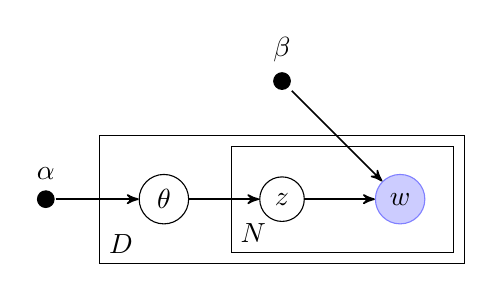
\begin{tikzpicture}
    [
      observed/.style={minimum size=15pt,circle,draw=blue!50,fill=blue!20},
      unobserved/.style={minimum size=15pt,circle,draw},
      hyper/.style={minimum size=1pt,circle,fill=black},
      post/.style={->,>=stealth',semithick},
    ]

    \node (w) [observed] at (0,0) {$w$};
    \node (z) [unobserved] at (-1.5,0) {$z$};
    \node (z-prior) [unobserved] at (-3,0) {$\theta$};
    \node (z-hyper) [label=above:$\alpha$] at (-4.5,0) {};
    \filldraw [black] (-4.5,0) circle (3pt);
    \node (w-hyper) [label=above:$\beta$] at (-1.5,1.5) {};
    \filldraw [black] (-1.5,1.5) circle (3pt);
    
    \path
    (z) edge [post] (w)
    
    (z-hyper) edge [post] (z-prior)
    (z-prior) edge [post] (z)

    (w-hyper) edge [post] (w)
    ;

    \node [draw,fit=(w) (z-prior), inner sep=14pt] (plate-context) {};
    \node [above right] at (plate-context.south west) {$D$};
    \node [draw,fit=(w) (z), inner sep=10pt] (plate-token) {};
    \node [above right] at (plate-token.south west) {$N$};

  \end{tikzpicture}
  \caption{Plate Diagram of LDA. For more information, see \cite{Blei:2003:LDA:944919.944937} }
  \label{fig:graphical-model}
\end{figure}

\section{Equations}

\subsection{Generative Process}
\begin{algorithmic}[1]
  \FOR{document $d_i$ in corpus $D$}
  \STATE Choose $\theta_i \sim \dir(\alpha) $
  \FOR{position $j$ in $d_i$}
    \STATE Choose a topic $z_j \sim \mult(\theta_i)$
    \STATE Choose a word $w_j$ from $p(w_j | z_j,\beta)$, a multinomial distribution over words conditioned on the topic and the prior $\beta$.
  \ENDFOR
  \ENDFOR
\end{algorithmic}

\bibliographystyle{plain}
\bibliography{tm}

\end{document}
